\documentclass[xcolor=dvipsnames]{beamer}
\usepackage[utf8]{inputenc}

\usepackage{tikz}
\usetikzlibrary{positioning, calc}

%------------------------------------------------------------
%Theme
\usetheme{Madrid}
\usecolortheme[named=CadetBlue]{structure}
\setbeamertemplate{caption}[numbered]
\setbeamertemplate{bibliography item}[text]
%------------------------------------------------------------

%------------------------------------------------------------
%Title page
\title{Reinforcement Learning (DQN)}
\author{Pierre Squarra}
\date{Cognitive Algorithms Seminar}

% Beginning of each section
\AtBeginSection[]
{
  \begin{frame}
    \frametitle{Outline}
    \tableofcontents[currentsection]
  \end{frame}
}
%------------------------------------------------------------

\begin{document}

{
\logo{
\includegraphics[height=1cm]{images/tu-berlin.png}}
\begin{frame}
  \titlepage
\end{frame}
}

% Outline
\begin{frame}{Outline}
\tableofcontents
\end{frame}
%---------------------------------------------------------

\begin{frame}{Learning in Dynamic Environments}
    \begin{columns}
        \begin{column}{0.5\textwidth}
            \begin{figure}
                \centering
                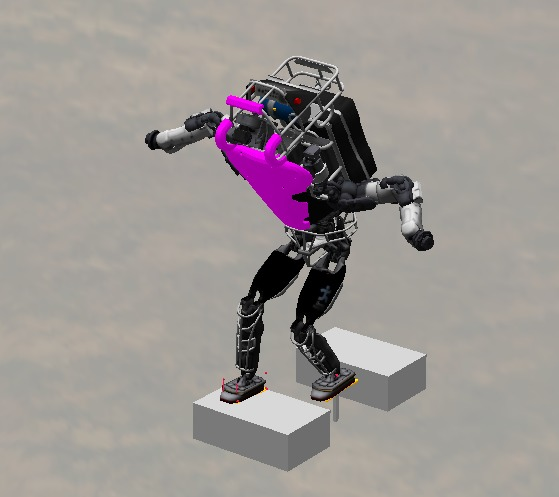
\includegraphics[width=0.9\textwidth]{images/atlas.jpg}
                \caption{Walking Robot \cite{wiedebach_walking_2016}}
                \label{fig:walking-robot}
            \end{figure}
        \end{column}
        \begin{column}{0.5\textwidth}
            \begin{figure}
                \centering
                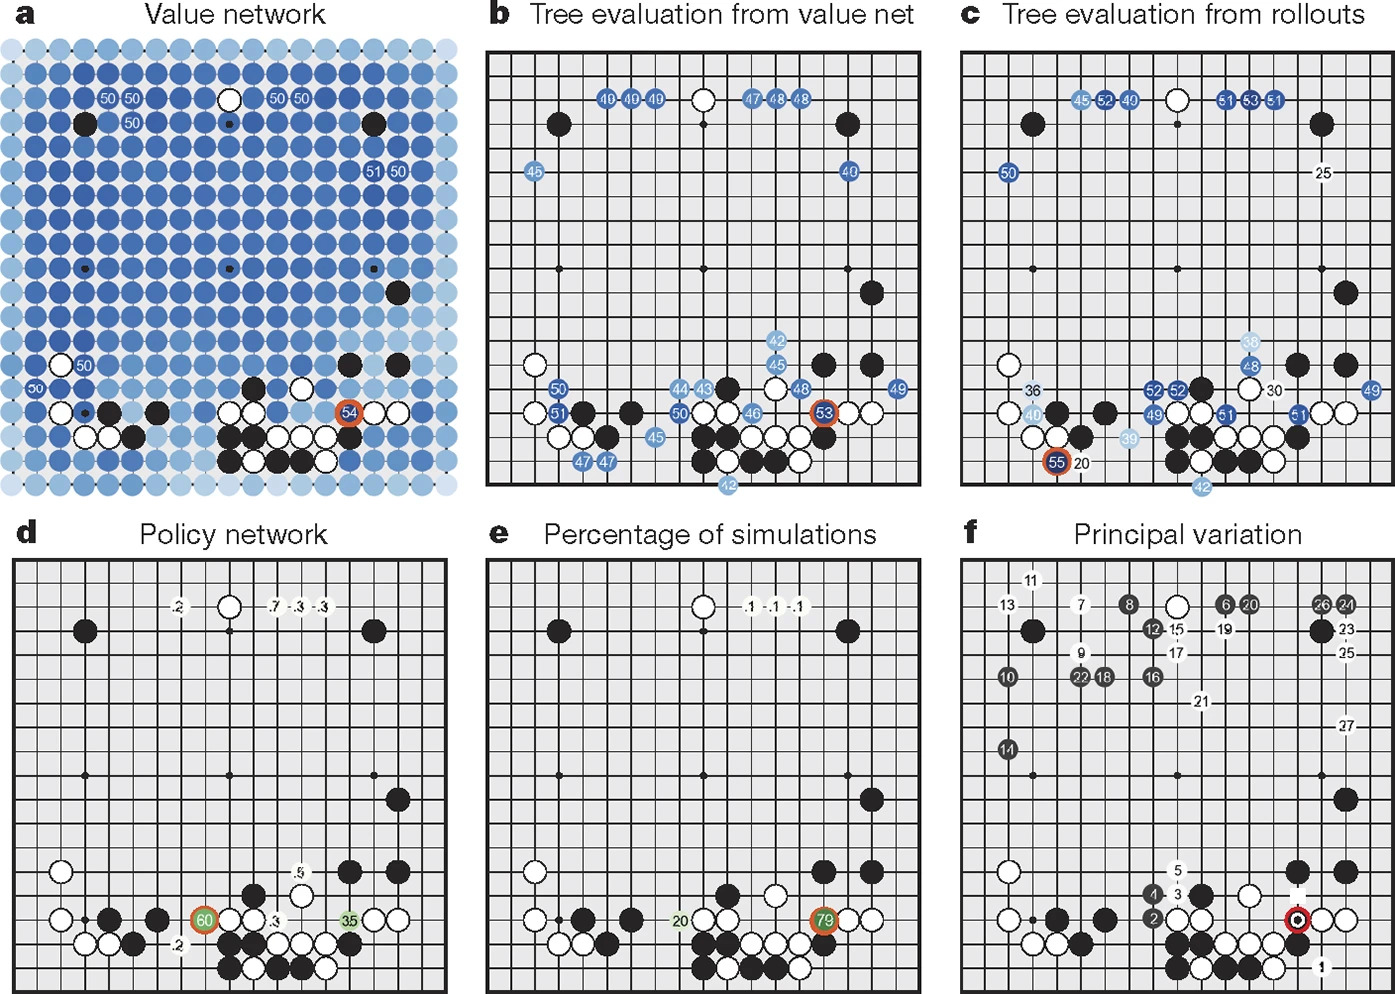
\includegraphics[width=0.9\textwidth]{images/alphago.jpg}
                \caption{AlphaGo \cite{silver_mastering_2016}}
                \label{fig:autonomous-driving}
            \end{figure}
        \end{column}
    \end{columns}
\end{frame}

%---------------------------------------------------------

\section{Reinforcement Learning}
\subsection{Agent-Environment Interface}
\begin{frame}{Agent-Environment Interface}
    \begin{minipage}[c][2cm][c]{\textwidth}
        \only<1>{\begin{description}[labelsep=2cm]
            \item[Agent:] Decision-maker taking actions
            \item[Environment:] World which the agent interacts with
        \end{description}}
        \only<2>{\begin{description}[labelsep=2cm]
            \item[Action:] Move the agent can make in the environment
            \item[Observation:] Agent's perception of the environment
        \end{description}}
        \only<3>{\begin{description}[labelsep=2cm]
            \item[State:] Current situation or configuration of the environment
            \item[Reward:] Scalar value given to an agent as feedback for its actions
        \end{description}}
    \end{minipage}
    
    \tikzset{
    block/.style={rectangle, draw, text width=6em, text centered, minimum height=3em},
    action/.style={rectangle, color=white, fill=structure, text width=7em, text centered, minimum height=2em, rounded corners=5pt}}
    
    \begin{figure}
        \begin{tikzpicture}[thick]
            % Nodes
            \node[block] (agent) {Agent};
            \node[block, right=5cm of agent] (environment) {Environment};
            \uncover<2->{\node[action, above=1cm of {$(agent)!0.5!(environment)$}] (actions) {Action};}
            \uncover<2->{\node[action, below=1cm of {$(agent)!0.5!(environment)$}] (observations) {Observation};}
            \uncover<2->{\node[below=0mm of actions] (action) {\small action $a_t$};}
            \uncover<3->{\node[above=0mm of observations] (new_state) {\small state $s_{t+1}$};}
            \uncover<3->{\node[below=0mm of observations] (reward) {\small reward $r_{t+1}$};}
            % Arrows
            \uncover<2->{\draw[-, color=structure] (agent.north) |- (actions.west);}
            \uncover<2->{\draw[->, color=structure] (actions.east) -| (environment);}
            \uncover<2->{\draw[-, color=structure] (environment.south) |- (observations.east);}
            \uncover<2->{\draw[->, color=structure] (observations.west) -| (agent.south);}
        \end{tikzpicture}
        \caption{The agent-environment interface \cite{amini_deep_2023}}
        \label{fig:agent-environment}
    \end{figure}
\end{frame}

\subsection{Returns and Value Functions}
\begin{frame}{Returns and Value Functions}
    \begin{itemize}
        \only<1>{\item \textbf{Goal:} maximize cumulative reward, called the \alert{return} \hfill\cite{sutton_reinforcement_2020}}
        \only<2->{\item \textbf{Goal:} maximize cumulative reward, called the \alert{discounted return} \hfill\cite{sutton_reinforcement_2020}}
    \end{itemize}
    \only<1>{\begin{equation*}
            G_t = R_{t+1} + R_{t+2} + R_{t+3} + \dots + R_T
    \end{equation*}}
    \only<2->{\begin{equation*}
            G_t = R_{t+1} + \gamma R_{t+2} + \gamma^2 R_{t+3} + \dots = \sum_{k=0}^{\infty} \boldsymbol{\gamma}^k R_{t+k+1} 
    \end{equation*}}

    \begin{itemize}
        \item<2-> $\boldsymbol{\gamma}$: discount factor; $0 \leq \gamma \leq 1$
    \end{itemize}
    
    \begin{columns}<3->
        \begin{column}{0.41\textwidth}
            \begin{block}{State-Value function \hfill \cite{sutton_reinforcement_2020}}
                \begin{equation*}
                    v(s) = \mathbb{E} [G_t \mid S_t = s]
                \end{equation*}
                How good it is for the agent to be in a given state
            \end{block}
        \end{column}
        \begin{column}{0.43\textwidth}
            \begin{block}{Action-Value function \hfill\cite{sutton_reinforcement_2020}}
                \begin{equation*}
                    q(s,a) = \mathbb{E} [G_t \mid S_t = s, A_t = a]
                \end{equation*}
                How good it is to perform a certain action in a given state
            \end{block}
        \end{column}
    \end{columns}
    \vspace{5mm}
    \begin{itemize}
        \item<3-> A \alert{policy} is a strategy that the agent follows to decide actions based on the current state $\pi(s) \rightarrow a$
    \end{itemize}
\end{frame}

%---------------------------------------------------------

\section{Basic Algorithms}
\subsection{Q-Learning}
\begin{frame}{Q-Learning}
    \begin{itemize}
        \item \alert{Q-Learning} uses a Q-table with $S \times A$ entries to store the expected rewards for state-action pairs
        \begin{equation*}
            Q(S_t, A_t) \leftarrow Q(S_t, A_t) + \alpha \underbrace{\Bigl[R_{t+1} + \gamma \max_a Q(S_{t+1}, a) - Q(S_t, A_t)\Bigr]}_\text{Bellman error} \cite{grosse_q-learning_2019}
        \end{equation*}
        \item The \alert{Bellman error} is the difference between the current estimate of the Q-value for a state-action pair and the "true" Q-value
        \item The learning rate $\boldsymbol{\alpha}$ determines how quickly the agent learns from its experiences
    \end{itemize}
\end{frame}

\subsection{Limitations of standard RL}
\begin{frame}{Limitations of standard RL}
    \begin{itemize}
        \item Curse of dimensionality
        \begin{description}
            \item[Problem:] Tabular methods are impractical
        \end{description}
        \item Generalization across states
        \begin{description}
            \item[Problem:] Fail to generalize across similar states
        \end{description}
        \item Continuous state and action spaces
        \begin{description}
            \item[Problem:] Designed for continuous domains
        \end{description}
    \end{itemize}
    \begin{block}{Solution}<2->
        Use a function approximator to estimate $Q(S,A)$
        \begin{itemize}
            \item[$\boldsymbol{\rightarrow}$] Deep Neural Network
        \end{itemize}
    \end{block}
\end{frame}

%---------------------------------------------------------

\section{Deep Q Networks}
\subsection{Workings of DQNs}
\begin{frame}{Deep Q Networks}
    \tikzset{
    input/.style={rectangle, draw, text width=3em, text centered, minimum height=2em},
    nn/.style={rectangle, color=white, fill=structure, text width=4em, text centered, minimum height=3em, rounded corners=5pt}}
    
    \begin{itemize}
        \item Extension of Q-Learning $\boldsymbol{\rightarrow}$ Estimate the optimal Q-function
    \end{itemize}
    \begin{columns}
        \begin{column}{0.48\textwidth}
            \begin{block}{Action $\boldsymbol{+}$ State $\boldsymbol{\rightarrow}$ Expected Return \hfill \cite{amini_deep_2023}}
                \begin{minipage}[c][2.5cm][c]{\linewidth}
                    \begin{tikzpicture}[thick]
                        \node[input] (state) {State};
                        \node[input, below=3mm of state] (action) {Action};
                        \node[nn, right=4mm of $(state.east)!0.5!(action.east)$] (nn) {Deep NN};
                        \node[right=4mm of nn] (output) {$Q(S,A)$};
                        \draw[->] (state.east) -- ++(2mm,0) |- (nn.west);
                        \draw[->] (action.east) -- ++(2mm,0) |- (nn.west);
                        \draw[->] (nn.east) -- (output.west);
                    \end{tikzpicture}
                \end{minipage}
            \end{block}
        \end{column}
        \begin{column}{0.48\textwidth}
            \begin{block}<2->{State $\boldsymbol{\rightarrow}$ Expected Return for each Action \hfill \cite{amini_deep_2023}}
                \begin{minipage}[c][2.5cm][c]{\linewidth}
                    \begin{tikzpicture}[thick]
                        \node[input] (state) {State};
                        \node[nn, right=4mm of state] (nn) {Deep NN};
                        \node[right=4mm of nn] (output2) {$Q(S,A_2)$};
                        \node[above=2mm of output2] (output1) {$Q(S,A_1)$};
                        \node[below=2mm of output2] (output3) {$Q(S,A_3)$};
                        \draw[->] (state.east) -- (nn.west);
                        \draw[->] (nn.east) -- ++(2mm,0) |- (output1.west);
                        \draw[->] (nn.east) -- ++(2mm,0) |- (output2.west);,
                        \draw[->] (nn.east) -- ++(2mm,0) |- (output3.west);
                    \end{tikzpicture}
                \end{minipage}
            \end{block}
        \end{column}
    \end{columns}
    \vspace{5mm}
    \uncover<3->{\begin{equation*}
        \mathcal{L(\theta)} = \Bigl\vert\Bigl\vert \underbrace{\Bigl(R_{t+1} + \gamma \max_a Q(S_{t+1}, a)\Bigr)}_\text{target} - \underbrace{Q(S_t, A_t)}_\text{predicted}\Bigr\vert\Bigr\vert^2 \hspace{5mm}\cite{amini_deep_2023}
    \end{equation*}}
\end{frame}

\subsection{Challenges in Deep Q Networks}
\begin{frame}{Frame Title}
    \begin{itemize}
        \item \textbf{Experience Replay}
        \begin{description}
            \item[Problem:] Correlation of states lead to inefficiencies and instability
            \item[Solution:] Randomly sample from a memory buffer to break correlation
        \end{description}
        \item \textbf{Target Network}
        \begin{description}
            \item[Problem:] Using the same network for selecting and evaluating actions makes it hard for the model to stabilize and converge
            \item[Solution:] Use a target network to evaluate actions
        \end{description}
    \end{itemize}
\end{frame}


%---------------------------------------------------------
\begin{frame}[allowframebreaks]{References}
\bibliographystyle{abbrv}
\bibliography{bibliography}
\end{frame}

\end{document}